\documentclass{article}
\usepackage{tmlr}
\usepackage{hyperref}
\usepackage{url}
\usepackage{booktabs}
\usepackage{graphicx}
\usepackage{amsmath}
\usepackage{amssymb}

\title{Frozen, Not Fine-tuned: A Controlled Evaluation of\\Geospatial Foundation Models for Agricultural Field Mapping}
\author{Anonymous authors\\Paper under double-blind review}

\begin{document}
\maketitle

\begin{abstract}
Most published evaluations of geospatial foundation models (GeoFMs) fine-tune them
end-to-end. For agricultural field-boundary mapping from Sentinel-2 this is unnecessary.
Across six countries, a frozen GeoFM backbone with a small decoder matches or
exceeds full fine-tuning, in-region for both Prithvi-EO-2.0 and TerraMind and
cross-region for Prithvi-EO-2.0, while training about $110\times$ fewer parameters. Fine-tuning also
reduces cross-region transfer. Two evaluation choices have hidden this result. First,
common benchmarks substitute a coarse land-cover proxy (ESA WorldCover ``cropland'')
for true field boundaries. Second, they compare GeoFMs against a per-pixel spectral
baseline. Both choices inflate the apparent GeoFM advantage. On identical pixels, a
supervised U-Net trained from scratch on true labels reaches 0.89 to 0.98 AUROC in
every region and matches frozen GeoFMs in five of six. India is the one exception,
where the GeoFM leads. The PANGAEA benchmark shows the same pattern on its
true-boundary task. The rule breaks under extreme label sparsity (around 0.1\%
positive pixels in Kenya); we report the boundary case and a ten-point evaluation
protocol.
\end{abstract}

\section{Introduction}
Two routes exist for adapting a pretrained geospatial foundation model (GeoFM) to a
new task: fine-tune the backbone end-to-end on target labels, or freeze it and train
a small head. Most GeoFM papers fine-tune. For agricultural field-boundary mapping,
that default is wrong.

Two conveniences shape most benchmarks in this area. The first is a land-cover
product (ESA WorldCover ``cropland'' at 10\,m) used as ground truth because true
field boundaries are scarce. The second is a per-pixel spectral baseline (a random
forest on band values) used as the non-FM comparison. This paper asks how those
choices affect model ranking, and what survives once they are corrected.

Section~\ref{sec:flaws} identifies two evaluation choices that bias these benchmarks;
PANGAEA \citep{pangaea} shows both effects independently. The first is the label
choice. Swapping true field boundaries for the WorldCover proxy raises a per-pixel
random forest from near chance to GeoFM-competitive on identical pixels and reverses
the apparent size bias. The second is baseline strength. A supervised U-Net trained
from scratch on true labels reaches 0.89 to 0.98 AUROC in every region and matches
frozen GeoFMs in five of six (India excepted). PANGAEA reports the same pattern: on
AI4SmallFarms, a from-scratch U-Net beats every evaluated GeoFM by about 20 mIoU,
while a GeoFM's headline win is measured against a proxy task.

Section~\ref{sec:spine} compares frozen-backbone GeoFM features (decoder trained on
frozen features) against full end-to-end fine-tuning in two settings. In-region,
across six regions and two GeoFMs, the frozen backbone matches or exceeds full
fine-tuning within $\pm 0.013$ AUROC on five of six regions. Cross-region (train on
one country, test on another with no target-region labels), frozen features transfer
at least as well as a from-scratch U-Net and substantially better than fine-tuning,
which overfits the source. The conclusion is the same in both settings: freeze the
backbone, train a decoder, do not fine-tune. Section~\ref{sec:boundary} reports the
one regime where the rule breaks (Kenya, around 0.1\% field-pixel coverage).
Section~\ref{sec:cost} quantifies the parameter savings. Section~\ref{sec:protocol}
gives a ten-point protocol.

\paragraph{Contributions.} (1) A same-pixel controlled apparatus that separates the
effect of label choice from that of baseline strength on GeoFM evaluation, applied
across six countries with Fields-of-The-World boundaries. (2) Evidence that those
two choices jointly account for the reported GeoFM advantage on field-boundary tasks,
corroborated by PANGAEA. (3) An in-region and cross-region finding that fine-tuning
does not improve over frozen features for field mapping, with one boundary condition
(extreme label sparsity) and a roughly $110\times$ cost gap. (4) A ten-point
evaluation protocol and a released, audited artifact.

\section{Related Work}
\label{sec:related}
\paragraph{Geospatial foundation models.} Recent GeoFMs pretrain on large unlabeled
satellite archives and are reused across tasks: masked-autoencoder models (SatMAE
\citep{satmae}, Scale-MAE \citep{scalemae}, Prithvi-EO \citep{prithvi}), contrastive
and multimodal models (CROMA \citep{croma}, Clay \citep{clay}, TerraMind
\citep{terramind}, AnySat \citep{anysat}), wavelength-conditioned models (DOFA
\citep{dofa}), spectral models (SpectralGPT \citep{spectralgpt}), pixel-timeseries
models (Presto \citep{presto}), and large supervised pretraining (SatlasPretrain
\citep{satlas}). Their downstream evaluations almost always fine-tune the backbone.
We question that default for field mapping.

\paragraph{Frozen features vs.\ fine-tuning.} Outside Earth observation, a
substantial literature documents that frozen pretrained features with a light head
are often competitive with full fine-tuning, and that fine-tuning can harm
out-of-distribution performance. \citet{kumar2022finetuning} show that fine-tuning
distorts pretrained features and underperforms frozen linear probing under
distribution shift, which is the pattern we observe across regions. Locked-feature
training \citep{zhai2022lit}, transfer studies
\citep{kornblith2019transfer,kolesnikov2020bit}, and the linear-probe evaluation of
self-supervised models \citep{he2022mae} all point in the same direction. We
establish the same pattern for geospatial field-boundary mapping, in and out of
distribution, with an explicit boundary condition and a cost analysis.

\paragraph{EO benchmarks and evaluation.} GEO-Bench \citep{geobench} and PANGAEA
\citep{pangaea} standardize GeoFM evaluation; we use PANGAEA's results as external
corroboration. Fields of The World \citep{ftw} supplies the true field boundaries
that let us replace land-cover proxies. We audit the evaluation choices (labels and
baselines) rather than propose a new model.

\section{Setup}
\label{sec:setup}
\paragraph{Data.} We use Sentinel-2 L2A chips paired with true field boundaries from
Fields of The World \citep{ftw} across six countries spanning smallholder to
industrial agriculture: India, Cambodia, Vietnam, Kenya, France, and the Netherlands.
For each chip we form two labels on the same pixels. The \textsc{true} label is 1
when the pixel lies inside an FTW field polygon, rasterized to the chip grid in the
chip's own CRS. The \textsc{proxy} label is 1 when the pixel is ESA WorldCover
``cropland'' (class~40, \citep{worldcover}). Figure~\ref{fig:labels} illustrates the
contrast.

\paragraph{Models.} Non-FM baselines: a per-pixel random forest on the 12 raw S2
bands, a $5\times5$ windowed random forest (300-d), and a from-scratch U-Net
\citep{unet} (31M parameters). GeoFMs: Prithvi-EO-2.0-300M \citep{prithvi} and
TerraMind \citep{terramind} (with Clay and AnySat for breadth), used in two modes.
Frozen: features extracted once, then a linear probe or a trained decoder.
Fine-tuned: backbone trained end-to-end with the same decoder.

\paragraph{Protocol.} All models are scored on the same held-out test pixels via a
chip-grouped split (no chip in both train and test; overlap $=0$; seed 20260514, 25\%
test). We report AUROC, mean$\pm$std over three training seeds. The apparatus, all
metric artifacts, and reproduction commands are released; every headline number was
independently recomputed from raw rasters and reproduced to three decimals
(Appendix~\ref{app:repro}).

\begin{figure}[t]
\centering
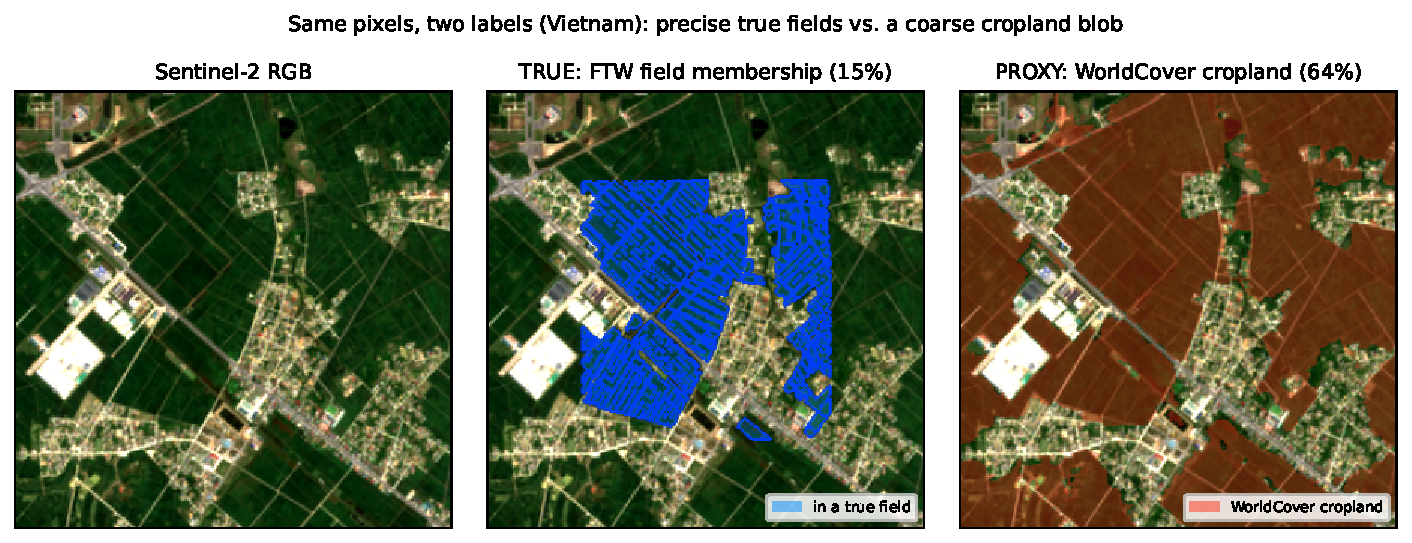
\includegraphics[width=0.92\linewidth]{figures/labels.pdf}
\caption{\textbf{The same pixels under two labels} (a Vietnam chip). Left: Sentinel-2
RGB. Middle: \textsc{true} FTW field membership (precise parcels). Right: WorldCover
``cropland'' \textsc{proxy} (a coarse blob). Benchmarking against the proxy quietly
replaces ``is this pixel in a field?'' (spatial) with ``is this pixel crop-like?''
(spectral), which a per-pixel baseline can solve.}
\label{fig:labels}
\end{figure}

\section{Two Evaluation Flaws}
\label{sec:flaws}
Table~\ref{tab:flaws} reports, per region, the per-pixel RF and the strong models
under both labels (\textsc{true}-label AUROC unless noted).

\begin{table}[t]
\centering\small
\caption{\textbf{Two evaluation flaws (true-label AUROC; mean over 3 seeds).} The
WorldCover proxy lifts the per-pixel RF from 0.55--0.82 (\textsc{true}) to 0.79--0.96
(\textsc{proxy}), making it foundation-model-competitive. A from-scratch U-Net on
\textsc{true} labels reaches 0.89--0.98 everywhere and matches frozen GeoFMs in five
of six regions (India excepted), so the reported ``GeoFM\,$\gg$\,baseline'' gap
mostly reflects the weak per-pixel baseline. ``frozen FM'' = best frozen GeoFM with a
linear probe; ``FT FM'' = fine-tuned Prithvi. U-Net and FT FM are mean$\pm$std over 3
seeds; RF and the linear probe are deterministic given the split. The
frozen-backbone-plus-decoder comparison is in Table~\ref{tab:spine}.}
\label{tab:flaws}
\begin{tabular}{lccccc}
\toprule
Region & RF \textsc{true} & RF \textsc{proxy} & U-Net & frozen FM & FT FM \\
\midrule
India        & 0.574 & 0.786 & 0.909\,{\scriptsize$\pm$.034} & \textbf{0.983} & 0.983\,{\scriptsize$\pm$.003} \\
Cambodia     & 0.550 & 0.900 & 0.948\,{\scriptsize$\pm$.001} & 0.924 & 0.949\,{\scriptsize$\pm$.000} \\
Vietnam      & 0.643 & 0.911 & 0.962\,{\scriptsize$\pm$.003} & 0.929 & 0.951\,{\scriptsize$\pm$.000} \\
Kenya        & 0.651 & 0.806 & 0.887\,{\scriptsize$\pm$.002} & 0.853 & 0.763\,{\scriptsize$\pm$.012} \\
France       & 0.695 & 0.959 & 0.977\,{\scriptsize$\pm$.000} & 0.961 & 0.978\,{\scriptsize$\pm$.001} \\
Netherlands  & 0.815 & 0.928 & 0.981\,{\scriptsize$\pm$.002} & 0.961 & 0.959\,{\scriptsize$\pm$.005} \\
\bottomrule
\end{tabular}
\end{table}

\paragraph{Flaw 1: proxy labels inflate weak baselines.} The proxy raises the
per-pixel RF by $+0.11$ to $+0.35$ AUROC in every region, turning a near-chance
field-membership predictor into one that rivals GeoFMs. The reason is that WorldCover
``cropland'' is spectrally separable while true field membership is a spatial
property. FTW-labeled fields cover a small fraction of a scene, while WorldCover
calls a majority of it cropland. The proxy therefore reframes the task as ``is this
managed land?'' rather than ``is this pixel in a field?'' (Appendix).

\paragraph{Flaw 2: weak baselines exaggerate the GeoFM advantage.} On \textsc{true}
labels a supervised U-Net reaches 0.89--0.98 AUROC in all six regions and matches
frozen GeoFMs in five of them. India is the exception: the GeoFM leads by about
0.07. The GeoFM advantage over the per-pixel RF is therefore largely an artifact of
the baseline. A per-pixel model cannot use spatial context, and a $5\times5$ windowed
RF closes only about 0.01 of the gap (Appendix). In-region, GeoFMs beat the U-Net in
only one of six regions (India), and that does not generalize: Cambodia, with
smaller fields than India, is a tie. The India win tracks the only high-variance
U-Net in the study ($\pm0.034$), not field size.

\paragraph{External corroboration (PANGAEA).} On AI4SmallFarms \citep{ai4smallfarms}
(manually digitized field boundaries), PANGAEA \citep{pangaea} reports a from-scratch
U-Net at 46.3 mIoU, beating every evaluated GeoFM (Prithvi 26.9, DOFA 27.1, Scale-MAE
21.5). Conversely, the Prithvi-EO-2.0 headline of $+8.1$ mIoU over a from-scratch
U-Net on multi-temporal crop segmentation \citep{prithvi} is measured against USDA
Cropland Data Layer proxy labels. Both flaws appear in the published literature,
independent of our apparatus.

\section{Fine-tuning Underperforms Frozen Features: In and Out of Distribution}
\label{sec:spine}
Holding the decoder, recipe, labels, and evaluation pixels fixed, Table~\ref{tab:spine}
compares frozen-backbone GeoFM features against full end-to-end fine-tuning.

\begin{table}[t]
\centering\small
\caption{\textbf{Fine-tuning does not help (true-label AUROC, mean$\pm$std, 3 seeds).}
\emph{Left, in-region :} frozen backbone + trained decoder vs.\
full fine-tuning of the same architecture (Prithvi). Frozen matches or beats
fine-tuning on five of six regions; only Kenya (extreme sparsity) favors fine-tuning.
\emph{Right, cross-region:} mean over 10 directed transfers (train country A, test
country B); frozen features transfer as well as a from-scratch U-Net and far better
than fine-tuning, which overfits the source.}
\label{tab:spine}
\begin{minipage}{0.56\linewidth}\centering
\textbf{In-region: frozen vs.\ fine-tune (Prithvi)}\\[2pt]
\begin{tabular}{lccc}
\toprule
Region & frozen-bb & full-FT & $\Delta$ \\
\midrule
India       & 0.983 & 0.983 & $+0.000$ \\
Cambodia    & 0.947 & 0.949 & $-0.002$ \\
Vietnam     & 0.954 & 0.951 & $+0.003$ \\
France      & 0.982 & 0.978 & $+0.004$ \\
Netherlands & 0.972 & 0.959 & $+0.013$ \\
Kenya       & 0.636 & 0.763 & $-0.127$ \\
\bottomrule
\end{tabular}
\end{minipage}\hfill
\begin{minipage}{0.4\linewidth}\centering
\textbf{Cross-region (10 transfers)}\\[2pt]
\begin{tabular}{lc}
\toprule
Model & mean AUROC \\
\midrule
frozen Prithvi  & \textbf{0.831} \\
frozen TerraMind & \textbf{0.828} \\
U-Net (scratch) & \textbf{0.825} \\
fine-tuned Prithvi & 0.777 \\
spectral RF & $\sim$0.50 \\
\bottomrule
\end{tabular}
\end{minipage}
\end{table}

\paragraph{In-region.} With the backbone frozen and only a decoder trained,
performance matches full fine-tuning on five of six regions (within $\pm0.013$ AUROC)
for both Prithvi and TerraMind (TerraMind: India $+0.001$, France $+0.006$).
Fine-tuning the 300M-parameter backbone gives no in-region gain. An
earlier apparent fine-tuning advantage came from an architecture confound: comparing
a fine-tune-plus-decoder against a frozen linear probe. Giving the frozen backbone
the same decoder removes the gap.

\paragraph{Cross-region.} Transferring across countries without target-region labels
(10 directed transfers among five regions; Vietnam is omitted from the transfer
subset), frozen GeoFM features (0.831 Prithvi, 0.828 TerraMind) transfer as well as a
from-scratch U-Net (0.825) and better than fine-tuned Prithvi (0.777).
Fine-tuning is the worst transferer in nearly every direction: it overfits the source
region. Frozen features win or tie 7 of 10 directed transfers; spectral features
collapse toward chance. We do not claim frozen features beat the U-Net on transfer
(they tie), but they achieve it with no target-region training and at a fraction of
the cost (Section~\ref{sec:cost}), and they avoid fine-tuning's degradation. Both
settings give the same conclusion: do not fine-tune the backbone.

\begin{figure}[t]
\centering
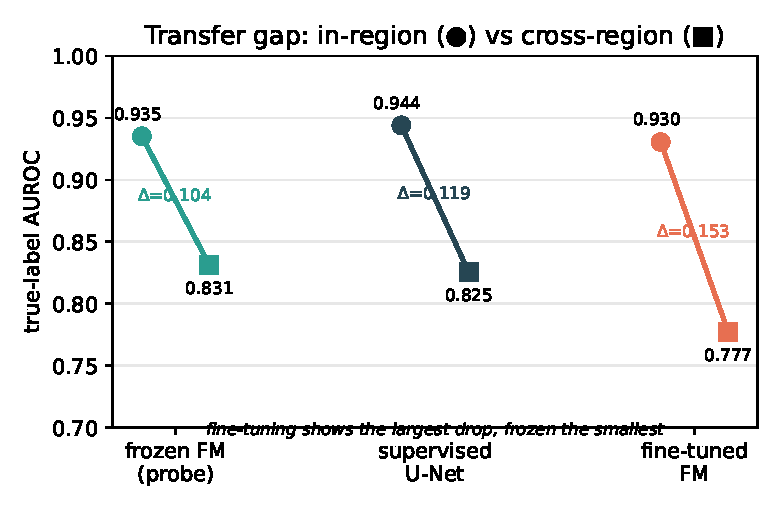
\includegraphics[width=0.6\linewidth]{figures/transfer_gap.pdf}
\caption{\textbf{Fine-tuning transfers worst.} In-region ($\bullet$) vs.\ cross-region
($\blacksquare$) mean AUROC per model class. The fine-tuned GeoFM has the largest
in-region-to-cross-region drop ($\Delta{=}0.15$); frozen features have the smallest
($\Delta{=}0.10$); the U-Net sits between the two.}
\label{fig:gap}
\end{figure}

\section{When the Rule Breaks: Characterizing the Boundary}
\label{sec:boundary}
Kenya is the one exception in both experiments: in-region, full fine-tuning beats the
frozen backbone ($\Delta=-0.127$), and cross-region the U-Net wins. Three properties
distinguish Kenya. First, label sparsity: Kenya's true-field-pixel coverage in
training masks is the lowest of any region at about 0.1\%, versus India 0.3\%,
Netherlands 3.8\%, France 11\%, Vietnam 18\%, Cambodia 23\%. This is not field size:
Cambodia has the smallest fields (79\% under 0.3 ha) but the highest coverage (23\%)
and obeys the rule, so the boundary tracks annotated-positive density, not parcel
size. Second, training-set size: Kenya has the fewest chips (155). Third, spatial fragmentation: Kenya's positive pixels form scattered micro-clusters rather than contiguous parcels, which leaves the decoder with far fewer within-field-interior contexts per chip than Cambodia or France. Under this combination,
frozen-feature decoders are unstable (seed std up to $\pm0.04$), and an end-to-end
CNN is the more robust choice. Threshold metrics sharpen the boundary: at probability
threshold 0.5, both the frozen probe and full fine-tune collapse to all-negative on
Kenya (F1$\,=\,$IoU$\,=\,$0; Appendix Table~\ref{tab:xmetrics}); only the supervised
U-Net recovers any positives (F1$\,=\,$0.115). Kenya is a boundary case across both
rank and threshold metrics, not an AUROC artifact.

We do not state a hard numeric threshold. With one region below about 0.2\% coverage,
the transition is an $n{=}1$ observation, and a precise cutoff would overclaim. A
working diagnostic instead: when annotated positives are very sparse
($\lesssim$0.2\% of pixels) and the training set is small, expect frozen-feature
decoders to become unstable, and prefer a from-scratch supervised CNN.
Practitioners can check their own positive rate and seed variance to decide.
Establishing the exact boundary is future work.

\section{Cost-Efficiency of Frozen Features}
\label{sec:cost}
Table~\ref{tab:cost} contrasts trainable parameters and per-region training cost. A
frozen backbone with a decoder trains 2.75M parameters versus 307M for full
fine-tuning, about $110\times$ fewer, while matching its accuracy. A frozen linear
probe trains about $10^3$ parameters in seconds on CPU and matches a 31M-parameter
U-Net trained on GPU. For cross-region deployment, the frozen probe needs no
target-region labels.

\begin{figure}[t]
\centering
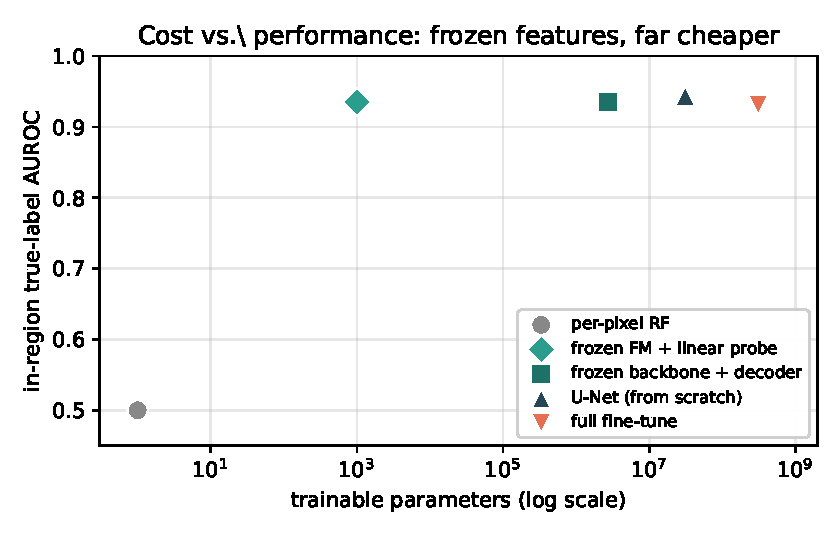
\includegraphics[width=0.62\linewidth]{figures/cost_perf.pdf}
\caption{\textbf{Cost vs.\ performance.} In-region AUROC against trainable parameters
(log scale). Frozen options (a $\sim$1K-parameter linear probe, or a 2.75M-parameter
decoder) sit at the cheap, high-accuracy corner, matching the 31M U-Net and the 307M
full fine-tune.}
\label{fig:cost}
\end{figure}

\begin{table}[t]
\centering\small
\caption{\textbf{Cost asymmetry.} Trainable parameters and per-region training cost.
Frozen options match full fine-tuning or the U-Net at a small fraction of the
trainable parameters.}
\label{tab:cost}
\begin{tabular}{lccc}
\toprule
Method & trainable params & per-region train & target labels \\
\midrule
per-pixel RF              & 0 (non-parametric) & seconds, CPU & yes \\
frozen FM + linear probe  & $\sim$1{,}000      & seconds, CPU & yes (source only, transfer) \\
frozen backbone + decoder & 2.75M              & $\sim$12 GPU-min & yes \\
supervised U-Net          & 31M                & $\sim$15 GPU-min & yes \\
full fine-tune (Prithvi)  & 307M               & $\sim$20 GPU-min & yes \\
\bottomrule
\end{tabular}
\end{table}

\section{A Corrected-Evaluation Protocol}
\label{sec:protocol}
We distill the study into a ten-point checklist for field-level GeoFM benchmarking.
\textbf{Labels:} (1) evaluate against true field boundaries, not a land-cover proxy;
treat proxy-only rankings as provisional. (2) Make the label comparison same-pixel
paired. \textbf{Baselines:} (3) include a strong task-specific supervised baseline
(U-Net), not only a per-pixel spectral model. (4) Report a frozen-feature probe and a
fine-tuned variant; do not assume fine-tuning helps. \textbf{Splits:} (5) group by
chip. (6) Add a scene or tile-disjoint split, and a cross-region split.
\textbf{Preprocessing:} (7) use each model's own normalization; exclude no-data.
\textbf{Statistics:} (8) cluster uncertainty at the chip level, use multiple seeds,
apply multiple-comparison correction. \textbf{Interpretation:} (9) run an
edge-vs-interior control before claiming boundary understanding. (10) Report across
field-size and label-sparsity regimes, and report trainable-parameter and compute
cost alongside accuracy.

\paragraph{Worked example: re-reading a published ranking.} The Prithvi-EO-2.0 report
\citep{prithvi} headlines a $+8.1$ mIoU win for the foundation model over a
from-scratch U-Net on multi-temporal crop segmentation. Protocol step (1) flags it
as provisional: the labels come from the USDA Cropland Data Layer, a per-pixel
land-cover proxy rather than true field boundaries, so the metric rewards
reproducing the proxy's per-pixel artifacts (Flaw 1). With true boundaries and a
strong baseline (steps 1 to 3), PANGAEA \citep{pangaea} reports on AI4SmallFarms
\citep{ai4smallfarms} (manually digitized parcels) a from-scratch U-Net at 46.3
mIoU, beating every evaluated GeoFM (Prithvi 26.9, DOFA 27.1, Scale-MAE 21.5).
Applying the protocol inverts the takeaway one would draw from the proxy-labeled
headline, using only published numbers.

\paragraph{Practitioner implications.} (i) Cost: a frozen backbone with a decoder
trains about $110\times$ fewer parameters than full fine-tuning, and a linear probe
about $10^3$ (Table~\ref{tab:cost}). It is cheaper to train, store, and version.
(ii) Label-scarce deployment: for a new region with no local labels, a
frozen-feature model trained elsewhere transfers as well as a region-specific U-Net
and better than a fine-tuned GeoFM. Fine-tuning should therefore be avoided
precisely when target labels are absent. (iii) Stability: frozen pipelines show
lower seed variance outside the extreme-sparsity regime. The default for
agricultural field mapping should be to extract frozen GeoFM features once, train a
small decoder, and skip fine-tuning unless positives are very sparse.

\section{Discussion, Limitations, Conclusion}
\label{sec:disc}
\paragraph{Scope.} Our claims are scoped to agricultural field-boundary mapping from
single-date Sentinel-2 with true field labels. They do not necessarily extend to
other tasks (e.g.\ crop-type, change detection), other sensors, or multi-temporal
regimes. GeoFM pretraining may help there.

\paragraph{Why not ``GeoFMs are useless.''} We do not argue against GeoFMs. We argue
that current evaluations overstate their advantage for in-distribution field mapping
with reasonable supervision, and that their practical value here is as frozen
feature extractors. They are cheap, stable, and transfer-competitive in that
configuration, rather than as backbones to fine-tune.

\paragraph{Limitations.} Four GeoFMs evaluated here (PANGAEA covers more, with the
same pattern); a single supervised architecture (PANGAEA independently replicates
with its own U-Net); FTW partial annotation in sparse regions (our sensitivity
analysis shows the conclusions are stable, Appendix); and the cross-region tie
rather than a win.

\paragraph{Connection to the broader foundation-model literature.} The cross-region
result empirically demonstrates, for geospatial models, what
\citet{kumar2022finetuning} established theoretically and for vision: fine-tuning
can distort pretrained features and underperform frozen probing under distribution
shift. The pattern recurs across modality, domain, and shift
type: multispectral satellite imagery rather than natural images; field-boundary
mapping rather than classification; geographic rather than corruption-based
distribution shift. This suggests the ``freeze, don't fine-tune'' recommendation
may extend to other Earth-observation tasks where labeled supervision is
regionally concentrated. Our apparatus is designed to test that hypothesis going
forward.

\paragraph{Conclusion.} For agricultural field mapping from Sentinel-2, the
recipe is: evaluate on true field boundaries, compare against a strong task-specific
supervised baseline, and deploy frozen GeoFM features rather than fine-tune the
backbone. Two evaluation choices, proxy labels and weak per-pixel baselines, have
made fine-tuned GeoFMs appear to dominate. The same-pixel controlled apparatus,
corroborated by PANGAEA, shows that a from-scratch supervised U-Net matches them in
all but one region (India) once both flaws are corrected. Across six regions, two foundation models, and both
in- and out-of-distribution settings, fine-tuning the backbone does not help, and
it hurts cross-region transfer. To our knowledge, this is the first controlled
multi-region demonstration of the result for geospatial field mapping. It holds
at roughly $110\times$ lower trainable-parameter cost. We release the apparatus, the ten-point protocol, and all
artifacts so that future GeoFM evaluations can avoid both flaws by construction.

\bibliographystyle{tmlr}
\bibliography{references}

\appendix
\section{Reproducibility and Controls}
\label{app:repro}
All experiments use the same canonical split (chip-grouped, seed 20260514, overlap
0). Headline numbers were independently recomputed from raw rasters and features
and reproduced to three decimals; label-to-imagery alignment was verified at 100\%
(every positive pixel inside a field polygon, every negative outside) in all six
regions. Controls: a per-pixel ablation ($1\times1$ convolutions) collapses to
$\approx$RF, and a $5\times5$ windowed RF gains only about 0.01 AUROC, which
confirms that the U-Net and GeoFM advantage is learned spatial context rather than
naive pooling. An edge-pixel control localizes the advantage to within-field
interior context. An FTW partial-labeling sensitivity test (restricting negatives
to high-confidence non-cropland) leaves the GeoFM true-task AUROC almost
unchanged (e.g.\ India Prithvi $0.983 \to 0.987$). Full cross-region transfer (all
10 directed pairs, three frozen GeoFMs) and per-seed tables are released with the
artifact. Code, the controlled-evaluation apparatus, and all metric artifacts (with
checksums and end-to-end reproduction commands) are available at
\url{https://anonymous.4open.science/r/frozen-not-finetuned-eval-C72B} (anonymized for
review; a Zenodo DOI and Croissant metadata will accompany the camera-ready).

\begin{table}[h]\centering\small
\caption{\textbf{Training recipe, held fixed across compared models.} All supervised
models share loss, augmentation, optimizer family, and schedule; only the backbone
treatment (frozen vs.\ fine-tuned vs.\ from-scratch) differs. Evaluation pixels and
the chip-grouped split are identical for every model and every seed.}
\label{tab:recipe}
\begin{tabular}{ll}
\toprule
Component & Setting \\
\midrule
Loss            & BCE (capped positive weight, $\le 50$) $+$ Dice \\
Optimizer       & U-Net: Adam, lr $10^{-3}$;\ \ GeoFM: AdamW (backbone $10^{-4}$, decoder $10^{-3}$) \\
LR schedule     & linear warmup (5 epochs, start factor 0.1) $+$ cosine decay \\
Augmentation    & random horizontal/vertical flips \\
Input           & U-Net: native chip, 12 S2 bands (reflect-padded); GeoFM: 224$\times$224 \\
Decoder         & GeoFM: shared 4-stage bilinear-upsample conv decoder (identical for frozen \& fine-tuned); U-Net: 4-level (31M) \\
Epochs          & U-Net 150 (from scratch); GeoFM fine-tune / frozen-probe 80 \\
Selection       & last epoch (no early stopping); mean$\pm$std over 3 training seeds \\
\bottomrule
\end{tabular}
\end{table}

\begin{table}[h]\centering\small
\caption{\textbf{Full cross-region transfer} (true-label AUROC, mean over 3 seeds;
train country A, test country B's canonical test pixels; cross-region transfer
covers a five-region subset, Vietnam omitted). Frozen GeoFM features are best or
tied-best in 7 of 10 directed transfers; fine-tuning (Prithvi-ft) is the worst
transferer in nearly all; the U-Net wins the three Kenya-involved transfers (the
extreme-sparsity boundary). The one direction in which fine-tuning helps Prithvi's
transfer is Cambodia$\rightarrow$India (Prithvi-ft 0.859 $>$ frozen Prithvi 0.832);
frozen TerraMind (0.879) is nonetheless highest there, so the ``don't fine-tune''
conclusion still holds at the model-class level.}
\label{tab:xfer-full}
\begin{tabular}{lcccc}
\toprule
A$\rightarrow$B & U-Net & Prithvi-ft & frozen-Prithvi & frozen-TerraMind \\
\midrule
India$\rightarrow$Cambodia      & 0.691 & 0.671 & 0.796 & 0.849 \\
Cambodia$\rightarrow$India      & 0.836 & 0.859 & 0.832 & 0.879 \\
France$\rightarrow$Netherlands  & 0.938 & 0.906 & 0.943 & 0.927 \\
Netherlands$\rightarrow$France  & 0.938 & 0.909 & 0.946 & 0.925 \\
India$\rightarrow$France        & 0.796 & 0.721 & 0.850 & 0.848 \\
France$\rightarrow$India        & 0.891 & 0.868 & 0.913 & 0.911 \\
India$\rightarrow$Kenya         & 0.690 & 0.576 & 0.721 & 0.748 \\
Kenya$\rightarrow$India         & 0.748 & 0.706 & 0.704 & 0.669 \\
Cambodia$\rightarrow$Kenya      & 0.883 & 0.839 & 0.853 & 0.808 \\
Kenya$\rightarrow$Cambodia      & 0.843 & 0.719 & 0.756 & 0.717 \\
\midrule
mean & 0.825 & 0.777 & 0.831 & 0.828 \\
\bottomrule
\end{tabular}
\end{table}

\begin{table}[h]\centering\small
\caption{\textbf{Spatial-pooling control (true-label AUROC).} A $5\times5$ windowed
random forest (300-d) gains only about 0.01 over the per-pixel RF and stays far
below the best foundation model. This confirms that the GeoFM and U-Net advantage
is learned spatial context, not naive local pooling. A per-pixel U-Net ablation
($1\times1$ convolutions, no spatial context) likewise collapses to $\approx$RF
(India 0.623, Vietnam 0.678).}
\label{tab:windowed}
\begin{tabular}{lccc}
\toprule
Region & per-pixel RF & windowed RF (5$\times$5) & best FM \\
\midrule
India       & 0.574 & 0.582 & 0.983 \\
Vietnam     & 0.643 & 0.657 & 0.929 \\
Kenya       & 0.651 & 0.641 & 0.853 \\
France      & 0.695 & 0.703 & 0.961 \\
Netherlands & 0.815 & 0.827 & 0.961 \\
\bottomrule
\end{tabular}
\end{table}

\begin{table}[h]\centering\small
\caption{\textbf{FTW partial-labeling sensitivity (true-label AUROC).} Restricting
negatives to high-confidence non-cropland (dropping ambiguous, possibly-unlabeled
field pixels) leaves the frozen-GeoFM score barely changed, while the
spectral RF rises. The GeoFM result is therefore not an artifact of FTW's
partial annotation: the RF's errors were concentrated on crop-like non-field pixels.
The large France RF gain ($0.695 \to 0.947$) reflects that many of its true-negatives
are spectrally crop-like (pasture, vineyards) and inseparable by a per-pixel RF.
Removing them leaves an easy spectral task. The GeoFM was already near-ceiling, so
it barely moves.}
\label{tab:partial}
\begin{tabular}{lcccc}
\toprule
Region & RF (all neg) & RF (high-conf) & Prithvi (all neg) & Prithvi (high-conf) \\
\midrule
India  & 0.574 & 0.665 & 0.983 & 0.987 \\
France & 0.695 & 0.947 & 0.961 & 0.968 \\
Kenya  & 0.651 & 0.698 & 0.766 & 0.774 \\
\bottomrule
\end{tabular}
\end{table}

\begin{table}[h]\centering\small
\caption{\textbf{Threshold-based metrics complement AUROC} (single seed, seed 0; F1
and IoU at probability threshold 0.5; AP is threshold-free). The AUROC story holds
across rank- and threshold-based metrics in dense-positive regions (Cambodia,
Vietnam, France, Netherlands), where U-Net, frozen probe, and full fine-tune cluster
within about 0.02 to 0.05 IoU. India keeps its single-region FM lead on AUROC and
AP; F1 and IoU are close across models there because positives are sparse (about
0.3\%). Kenya (about 0.1\% positives) shows the sharpest gap: both the frozen probe
and the full fine-tune collapse to F1$=$IoU$=$0 at the standard threshold, and AP
drops to 0.32 to 0.38, while the supervised U-Net retains AP$=$0.58 and F1$=$0.115.
The supervised CNN is therefore the more robust choice in the extreme-sparsity
regime, across every metric and not only AUROC. ``Frozen'' = Prithvi backbone
frozen, decoder trained (apples-to-apples vs.\ full fine-tune).}
\label{tab:xmetrics}
\begin{tabular}{llcccc}
\toprule
Region & Model & AUROC & AP & F1 & IoU \\
\midrule
India       & U-Net   & 0.960 & 0.893 & 0.583 & 0.412 \\
India       & Frozen  & 0.985 & 0.972 & 0.573 & 0.401 \\
India       & Full-FT & 0.981 & 0.971 & 0.617 & 0.446 \\
\midrule
Cambodia    & U-Net   & 0.951 & 0.927 & 0.914 & 0.842 \\
Cambodia    & Frozen  & 0.948 & 0.913 & 0.918 & 0.848 \\
Cambodia    & Full-FT & 0.942 & 0.904 & 0.916 & 0.846 \\
\midrule
Vietnam     & U-Net   & 0.957 & 0.938 & 0.916 & 0.845 \\
Vietnam     & Frozen  & 0.954 & 0.927 & 0.913 & 0.839 \\
Vietnam     & Full-FT & 0.951 & 0.920 & 0.907 & 0.831 \\
\midrule
Kenya       & U-Net   & 0.891 & 0.583 & 0.115 & 0.061 \\
Kenya       & Frozen  & 0.667 & 0.316 & 0.000 & 0.000 \\
Kenya       & Full-FT & 0.757 & 0.375 & 0.000 & 0.000 \\
\midrule
France      & U-Net   & 0.977 & 0.962 & 0.942 & 0.890 \\
France      & Frozen  & 0.982 & 0.972 & 0.921 & 0.853 \\
France      & Full-FT & 0.978 & 0.971 & 0.906 & 0.829 \\
\midrule
Netherlands & U-Net   & 0.982 & 0.980 & 0.892 & 0.805 \\
Netherlands & Frozen  & 0.971 & 0.966 & 0.818 & 0.692 \\
Netherlands & Full-FT & 0.950 & 0.953 & 0.788 & 0.650 \\
\bottomrule
\end{tabular}
\end{table}
\end{document}
